%!TEX root = ../dissertation.tex

\chapter{DMNApp: An Android Application}

\newthought{To evaluate the model on the wild}, and to provide some perspectives on the real-world applications of this problem, a frontend client for this task is proposed. As most image-based applications, it is necessary to acknowledge and recognize some of the design requirements involved in the implementation of such programs. In this case, for testing and evaluation purposes it has been decided to target a mobile application as final device frontend, as it allows the final users to test the DMN characteristics in-place, without having to upload an stored image onto a different web platform. Also, it is desired that the final application does integrate with native hardware devices, such as the device integrated camera(s), the microphone and additionally, access to the native localization services provided via GPS/GLONASS/GALILEO or via IP.

The main motivation behind this development consists in providing the building blocks necessary to design and build mobile applications that can be used to test computer vision models on the wild, as a generic proof-of-concept backend framework to provide Computer Vision services is proposed. On the present example and more specifically to this application, we use these set of building blocks to generate a visualization application for segmentation models, and more specifically, for language-based image segmentation tasks. It is necessary to add that this aplication can be extended to sort and categoriize images by more strong natural language criterions, instead of using object tags as most current applications do, it is possible to filter images based on a object referral expression, however, due to time constraints, this application is out of the scope of the present implementation.

\begin{figure}[!htbp]
    \centering
    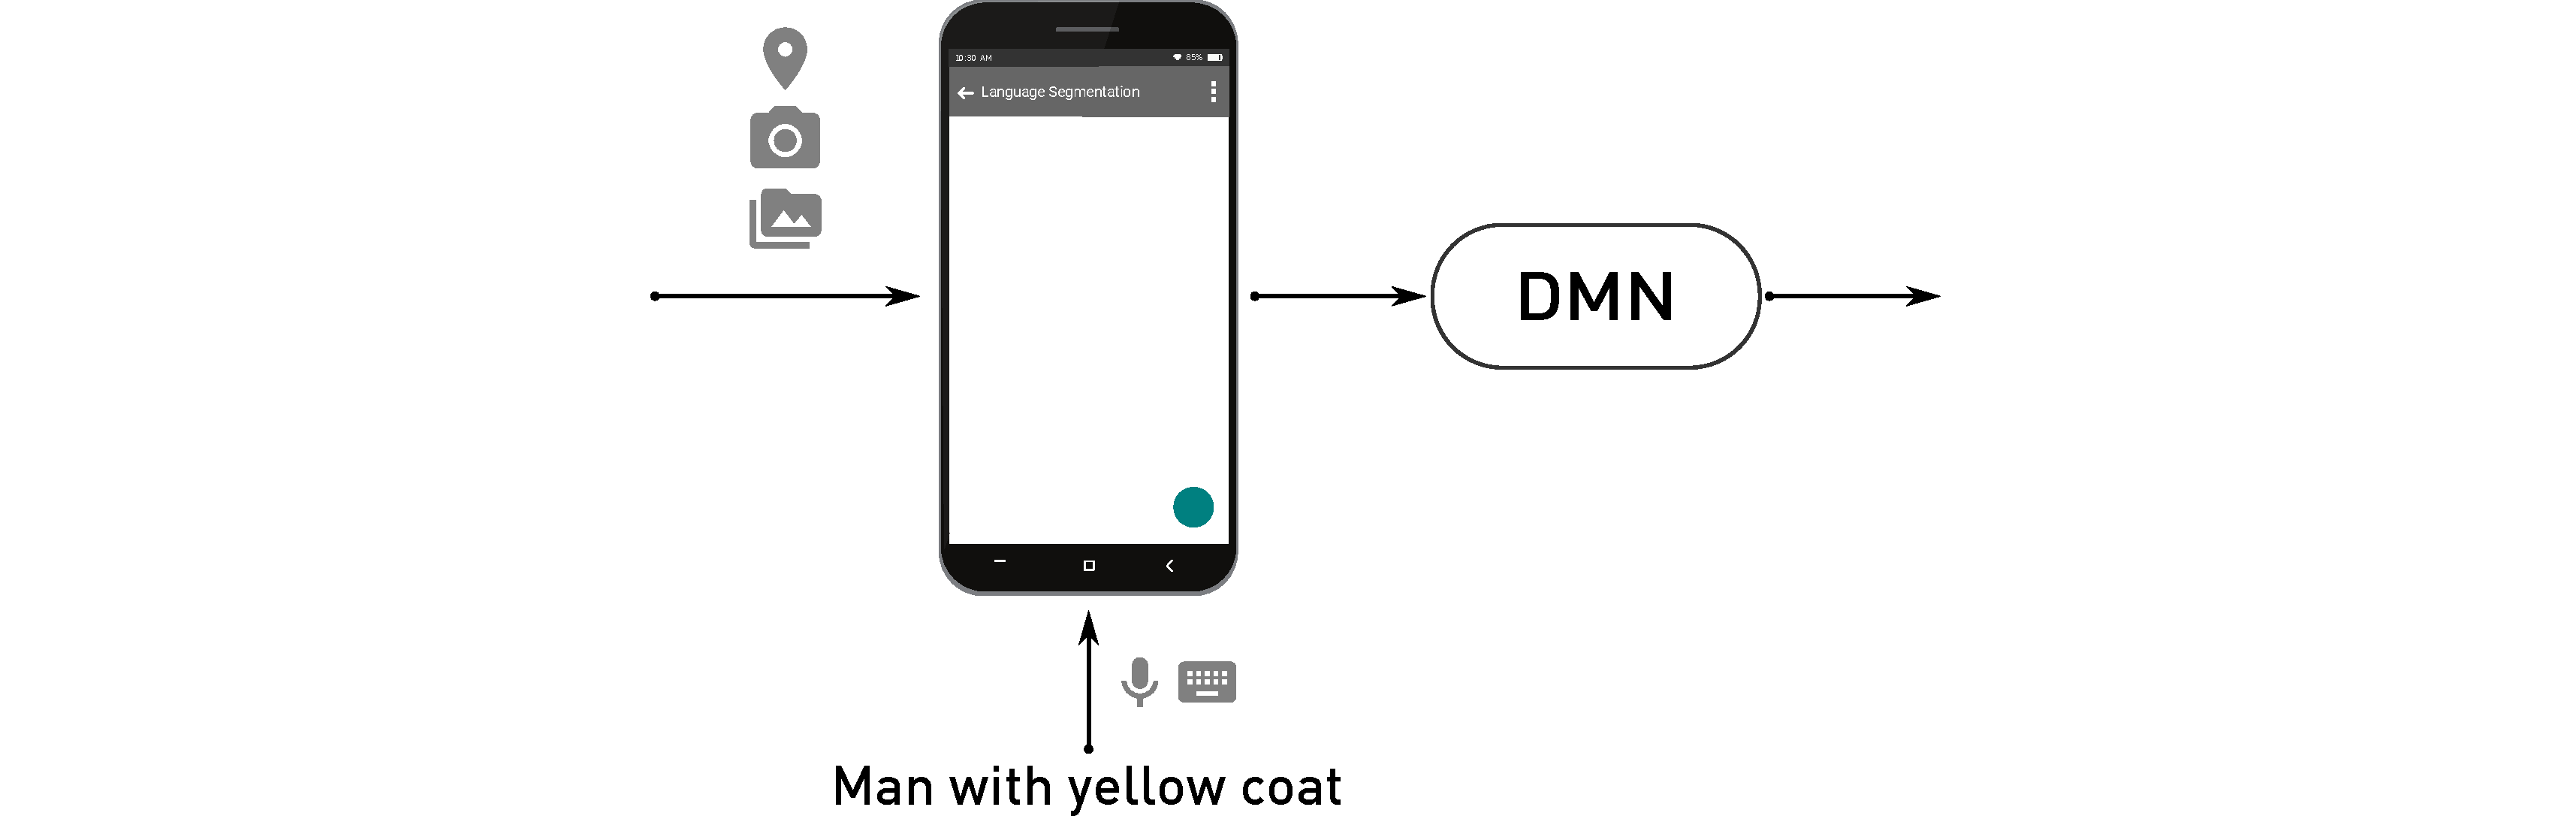
\includegraphics[width=\textwidth]{./figures/dmn_app/App_Overview.pdf}
    \caption{DMNApp general overview}
    \label{Fig:App_Overview}
\end{figure}

On Figure~\ref{Fig:App_Overview}, a summary of the general overview of the application is presented, describing the interaction between different device hardware/software elements, such as the camera/gallery to adquire an image and the microphone/keyboard to get a query phrase that is going to be processed by the DMN. As a result, the user can visualize and threshold the final segmentation using different values, the visualization can be customized by choosing different mask colors or by displaying the final result as a heatmap on different colormaps. Finally, the user can export a result to an image or share it with another application installed.

\section{Backend Architecture}
To process and handle multiple segmentation requests concurrently, a high scalable, fault-tolerant and high «performant» architecture is proposed. This architecture, as seen on Figure~\ref{Fig:Backend_Overview} comprises different servers and external services; for instance, the reference implementation\footnote{\url{https://github.com/andfoy/query-objseg-server}} comprises two servers, one to attend the final devices' requests (Frontend) and another one (Backend) to process the actual requests by running the DMN model hosted on a GPU. 

With respect to the external services used to communicate all three nodes, the architecture employs AWS S3 to store all the image requests, as well the raw segmentation masks responses. Also, it uses Firebase to handle incoming requests registration and storage, and also to notify end devices by using the Firebase Cloud Messaging (FCM) system, which enables the service to communicate asynchronously with a mobile device that starts a request and notify the completion of its petition.

\begin{figure}[!htbp]
    \centering
    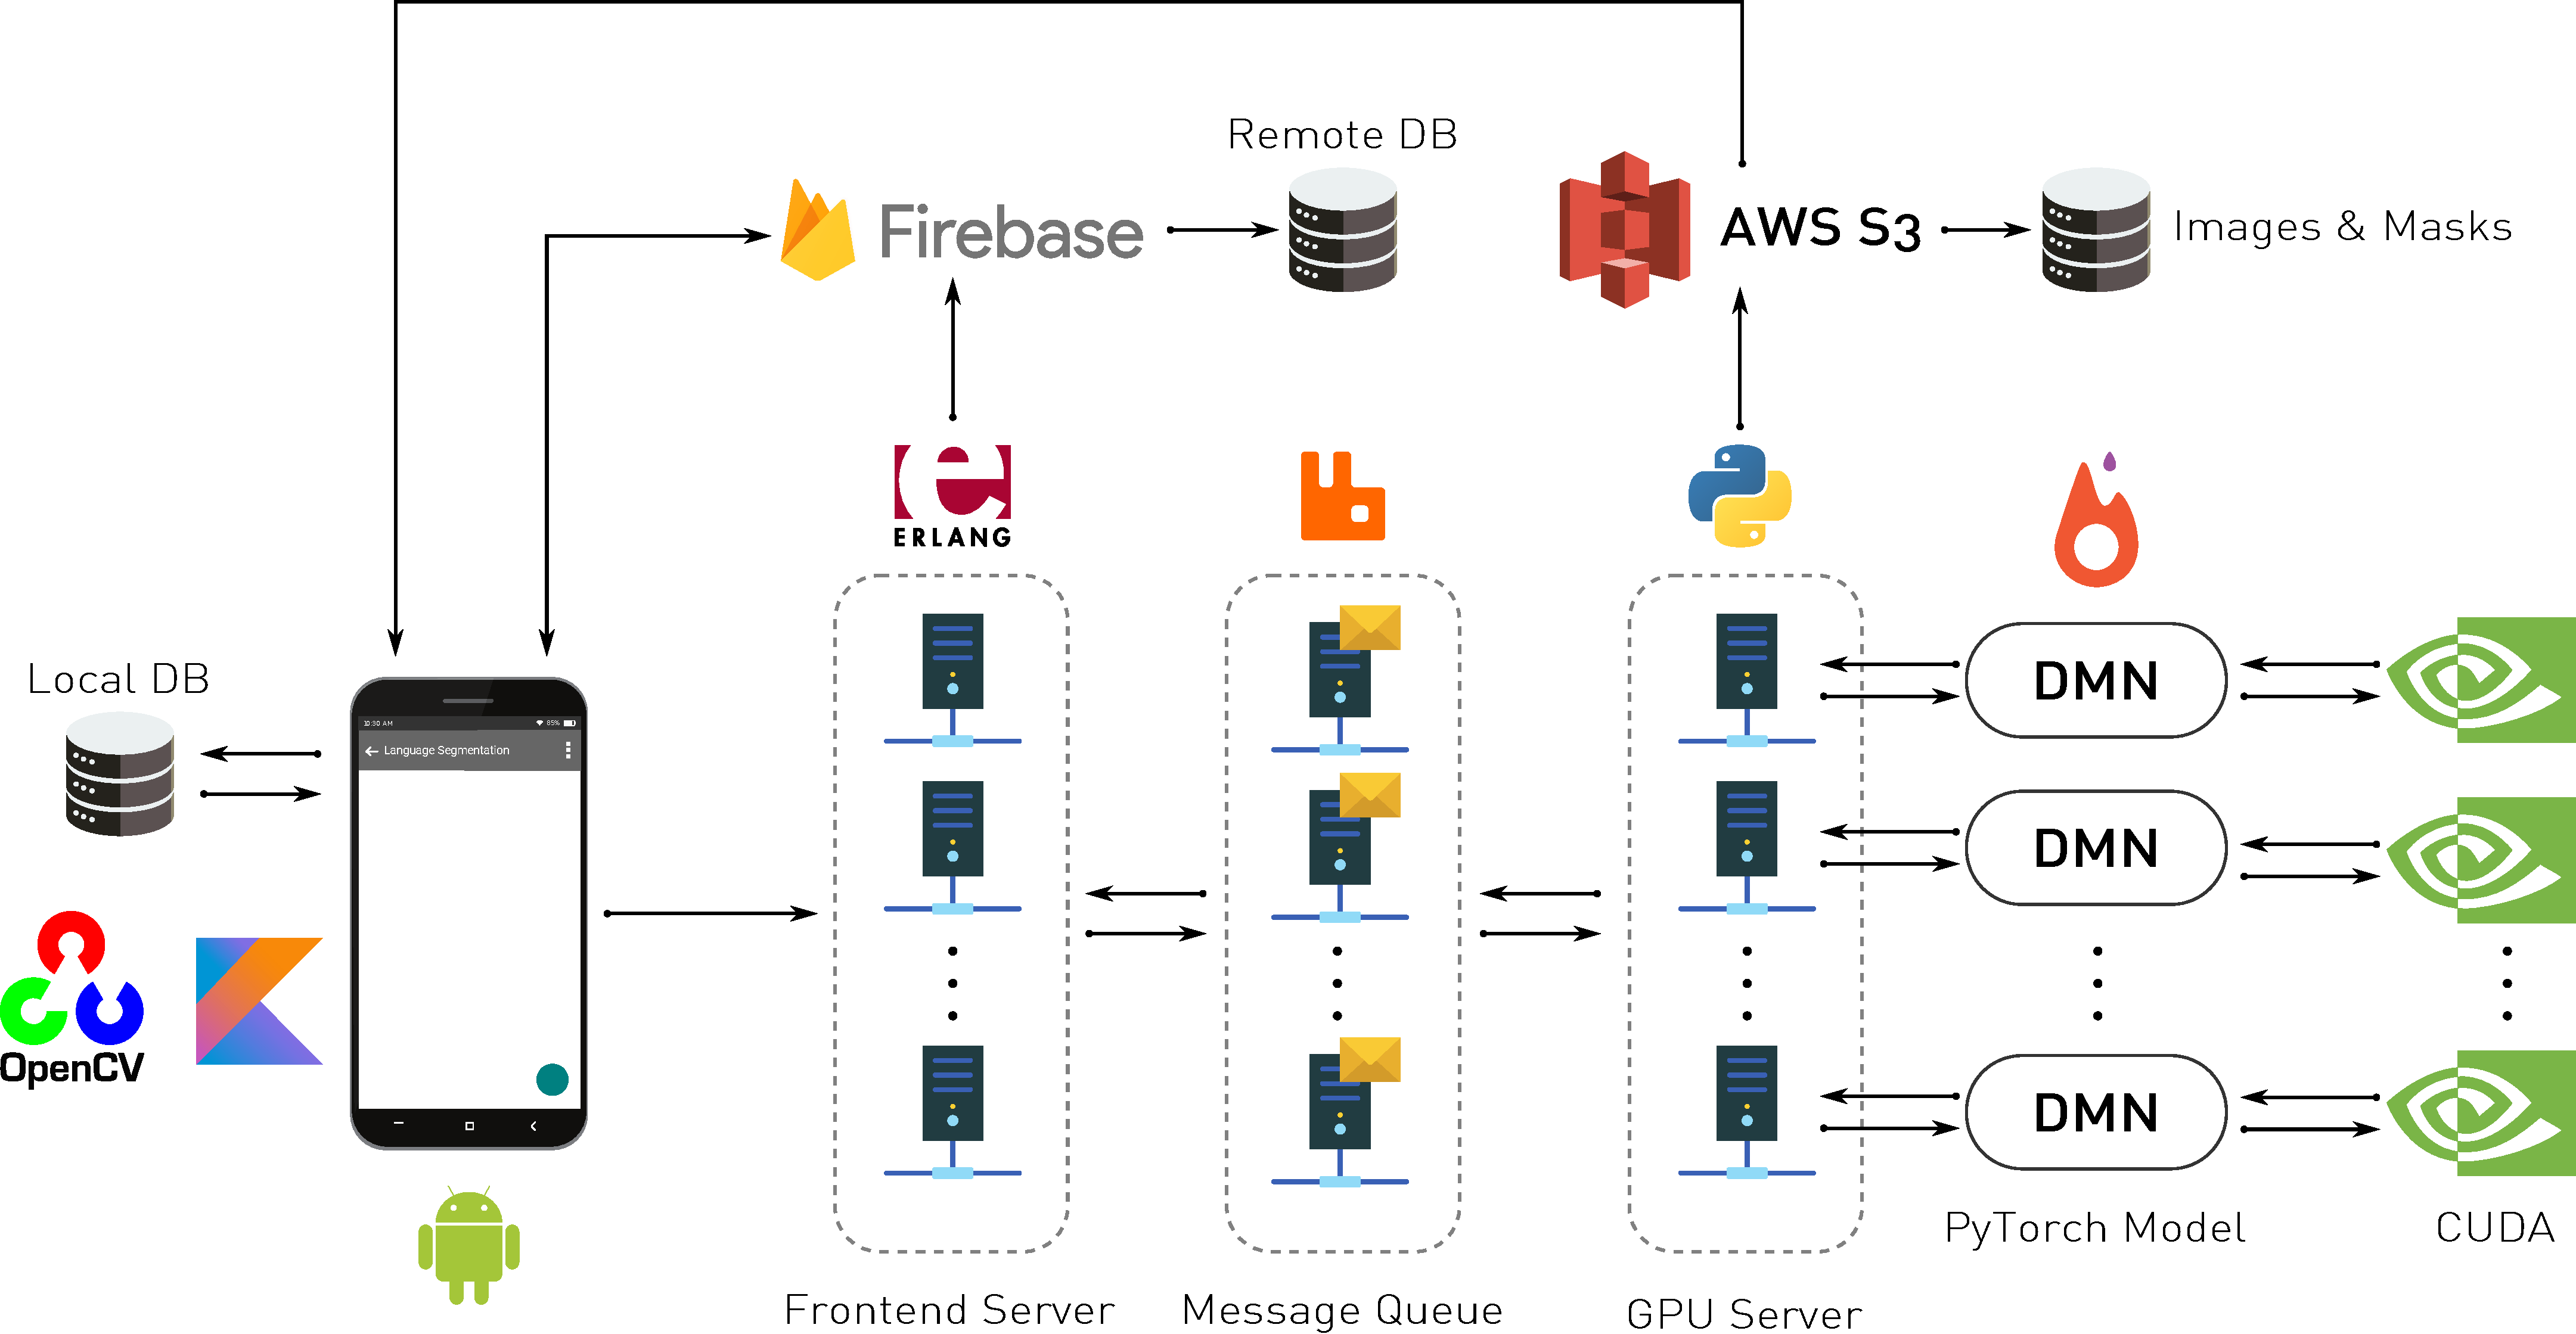
\includegraphics[width=\textwidth]{./figures/dmn_app/Backend_Overview.pdf}
    \caption{DMNApp backend architecture overview depicting the frontend server nodes, the messaging server nodes and the backend server nodes, alongside all the cloud services used additionally}
    \label{Fig:Backend_Overview}
\end{figure}

The frontend server consists of a complete Erlang stack that handles the following data flows: Device registration and identification, initial image segmentation request registration and result streaming to Firebase. By using Erlang\footnote{\url{https://www.erlang.org/}}, it is possible to guarantee design requirements related to performance, failure tolerance and availability\footnote{Erlang is known for its 9 nines availability figures}. For instance, the Erlang server can be replicated across a set of distributed nodes, such that it can handle multiple requests concurrently. As the requests have no state, all nodes can operate asynchronously without any interdependence between them. Also, this property assures that the server does not have to persist any information into disk, which represents one of the hallmark bottlenecks on most web servers, this in turn, enables us to use a in-memory database (Mnesia) to keep track of connected devices and requests that are pending of response by the backend server. 

To communicate both servers, the architecture proposed makes use of a broker server that runs RabbitMQ\footnote{\url{https://www.rabbitmq.com/}}, a messaging queue service also implemented on Erlang, thus satisfying also high performance, high availavility and multiple node replication. The messaging system is one of the core modules of the distribution system, as it allows to decouple a federation frontend servers from a cluster of backend processing servers. Also, the messaging system allows to replicate and parallelize the final processing servers, as they connect to a single request message queue, \textit{i.e.,} Any connected server is able to receive segmentation requests. Finally, this component enables the architecture to guarantee asynchronous behaviour, by queuing incoming requests; if a server is not available, then the request remains stored until it can be resolved. This implies that the unavailability of the backend server does not cause a failure of a request.

Finally, the backend server is the core processing node of the proposed architecture, this server, based on Python (Tornado Web Server\footnote{\url{http://www.tornadoweb.org/en/stable/}}) does run on the final GPU machines. Each server is asynchronous as well, which means that it can handle multiple requests concurrently. The server does take an incoming request from the message broker and processes its corresponding (image, query) pair using the DMN reference implementation written on PyTorch.

After processing a request and obtaining its corresponding segmentation map, the backend server does proceed to upload the input image and its result to S3, then it notifies to the frontend server of the request completion (Via RabbitMQ), which in turn does store the request on Firestore and sends a notification via FCM to the device that did initiate the request. Due to the asynchronous nature of the processing pipeline, a device only gets information about any request after it receives the completion notification, and therefore is not blocked after issuing a request.

It is necessary to note that the proposed architecture and servers are generic and transverse to any Deep Learning application that requires processing in a external server only by changing the model that the backend server uses to process information from different inputs given. Also, this backend can be used by different endpoint applications, such as mobile apps and web clients, as long as they can perform HTTP requests to the frontend server(s) and receive asynchronous notifications via FCM. 

\section{Android Application Implementation}
The reference Android application implementation\footnote{\url{https://github.com/andfoy/query-objseg-android}} is written on Kotlin\footnote{\url{https://kotlinlang.org/}} and it comprises several functions and activities that enable an user to do any of the following case uses:
\begin{enumerate}
    \item Request a segmentation based on an image and a query phrase \label{case:create}
    \begin{enumerate}
        \item Get image from Gallery/Camera \label{subcase:cam}
        \item Get user input using the Keyboard/Microphone
        \label{subcase:query_input}
        \item Get user geographical location (Optional)
        \label{subcase:gps}
    \end{enumerate}
    \item Delete a segmentation
    \item Visualize a segmentation result
    \begin{enumerate}
        \item Threshold mask with certain confidence value
        \label{subcase:thresh}
        \item Visualize mask on heatmap mode
        \label{subcase:vis_heatmap}
        \begin{enumerate}
            \item Select different colormaps
            \label{subsubcase:colormap}
        \end{enumerate}    
        \item Visualize mask as a contour overlay over the original image
        
        \begin{enumerate}
            \item Change overlay contour color
        \end{enumerate}
        \item Export visualization result
        \begin{enumerate}
            \item Save as image
            \item Send result image to other app
        \end{enumerate}
    \end{enumerate}
    \item Visualize segmentation localization on a map 
\end{enumerate}

For each use case, the app defines a different view designed taking into account Material Design's\footnote{\url{https://material.io/design/}} guidelines, therefore respecting the suggested Android look-and-feel. For instance, on Figure~\ref{subfig:app_main}, it is possible to observe an empty \texttt{RecyclerView} with a \texttt{FloatingActionButton} that allows users to create a new segmentation request based on images taken from the camera or the system gallery (Use case \ref{subcase:cam}), as shown on Figure~\ref{subfig:app_img_src}. 

\begin{figure}[!htbp]
    \centering
    \begin{multicols}{2}
    \begin{subfigure}[b]{\columnwidth}
            \centering
            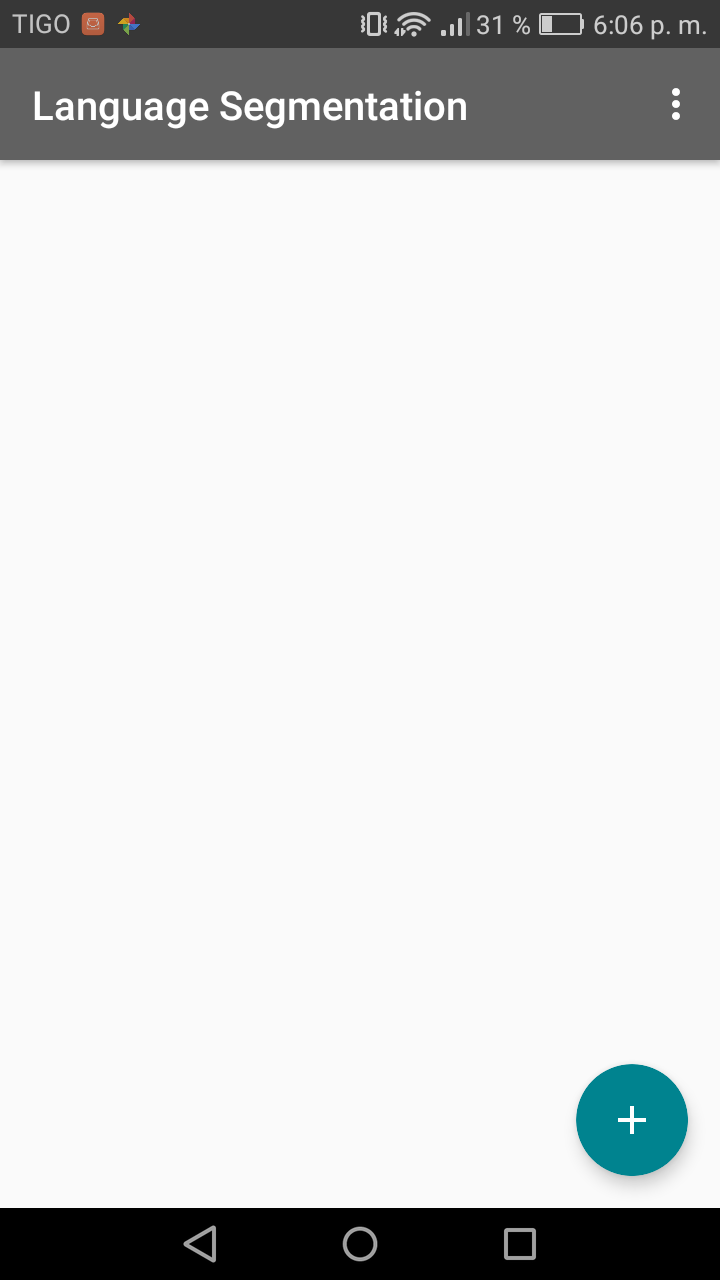
\includegraphics[width=\textwidth]{./figures/dmn_app/views/1.png}
    \subcaption{Main app activity view}
    \label{subfig:app_main}
    \end{subfigure}
    
    \begin{subfigure}[b]{\columnwidth}
            \centering
            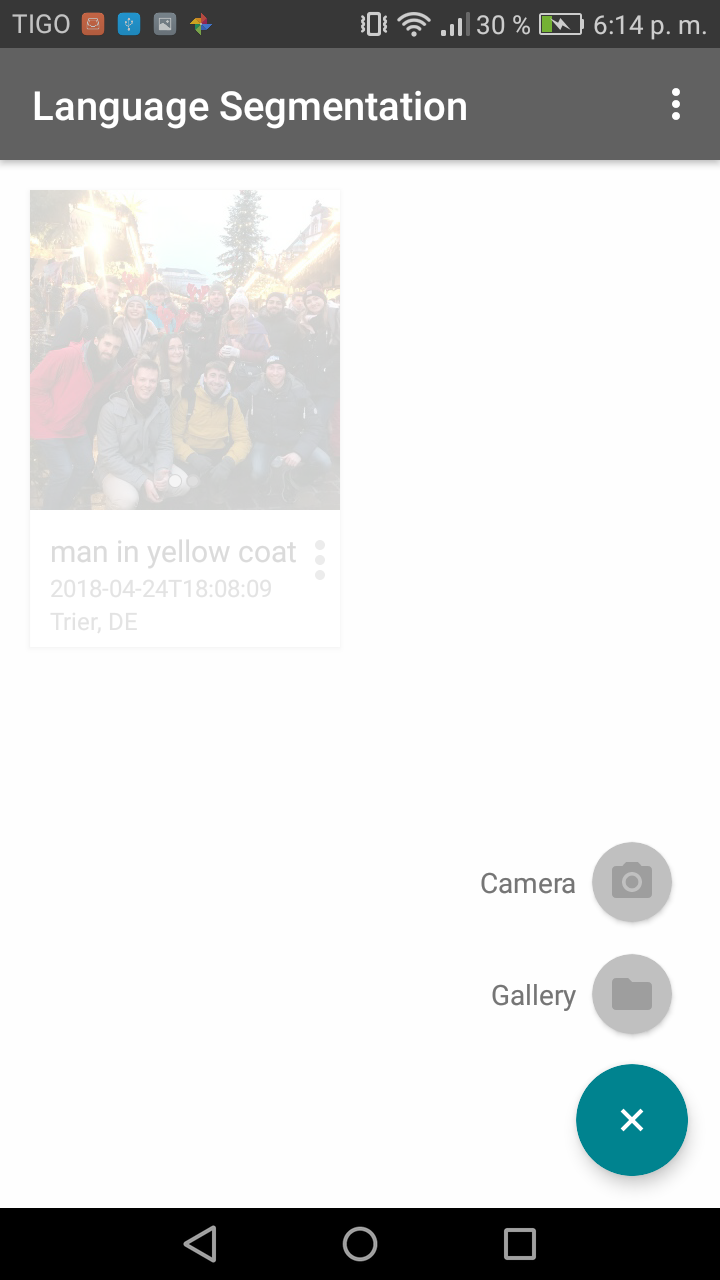
\includegraphics[width=\textwidth]{./figures/dmn_app/views/2.png}
    \subcaption{Use case \ref{subcase:cam}: DMNApp image source options selection menu}
    \label{subfig:app_img_src}
    \end{subfigure}
    \end{multicols}
    
    \caption{Main DMN Activity GUI depicting a Floating Action Button \ref{subfig:app_main} and its options \ref{subfig:app_img_src}}
    \label{Fig:App_Main}
\end{figure}

After picking one of the options, the user will be redirected to the external application that provides the option required, if an image is selected, then the user is taken to the image preview Activity (Figure~\ref{subfig:image_pre}), where it is not only possible to review the image to be sent, but it also allows to input an input query phrase, using a text input box that allows both traditional text input via a keyboard, and speech to text input\footnote{Using Google voice services} (Use case \ref{subcase:query_input}), as shown on Figure~\ref{subfig:mic_input}. Additionally, the user can add a localization reference to the request (Figure~\ref{subfig:loc}) based on a custom position or based on the current device position, obtained via GPS/IP.

\begin{figure}[!htbp]
    \centering
    \begin{multicols}{3}
    \begin{subfigure}[b]{\columnwidth}
            \centering
            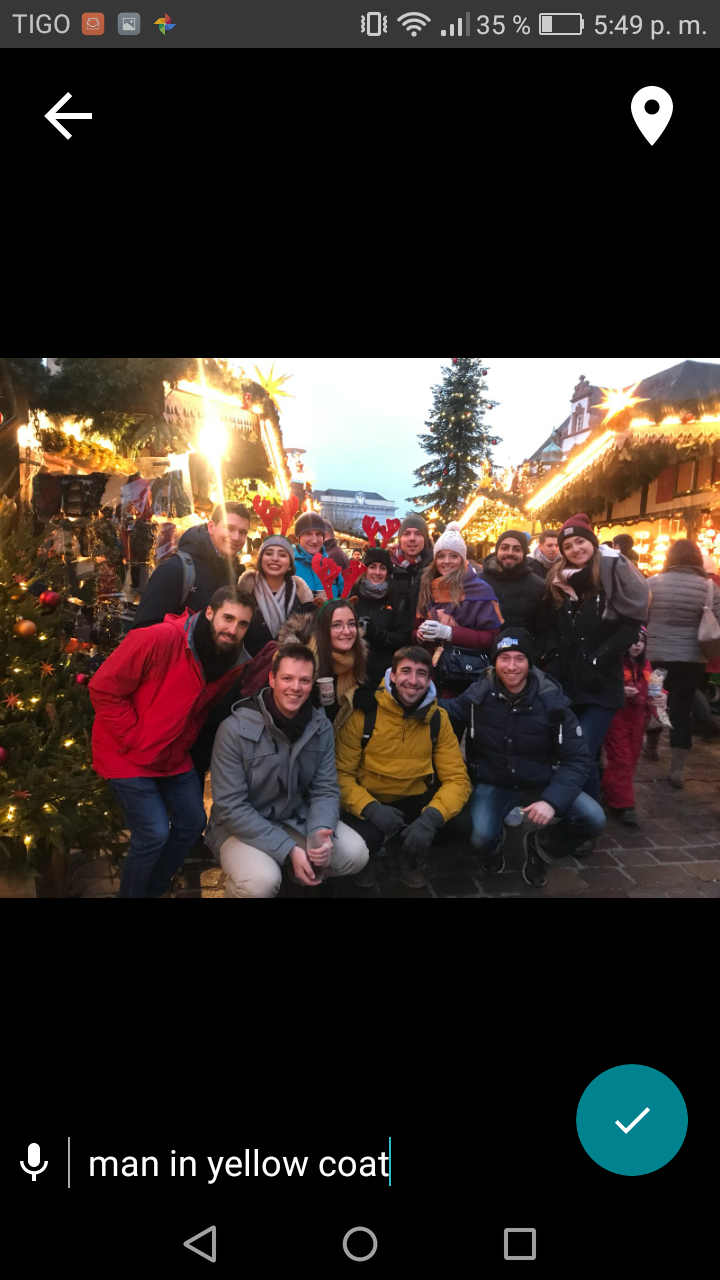
\includegraphics[width=\textwidth]{./figures/dmn_app/views/3.png}
    \subcaption{Image preview activity}
    \label{subfig:image_pre}
    \end{subfigure}
    
    \begin{subfigure}[b]{\columnwidth}
            \centering
            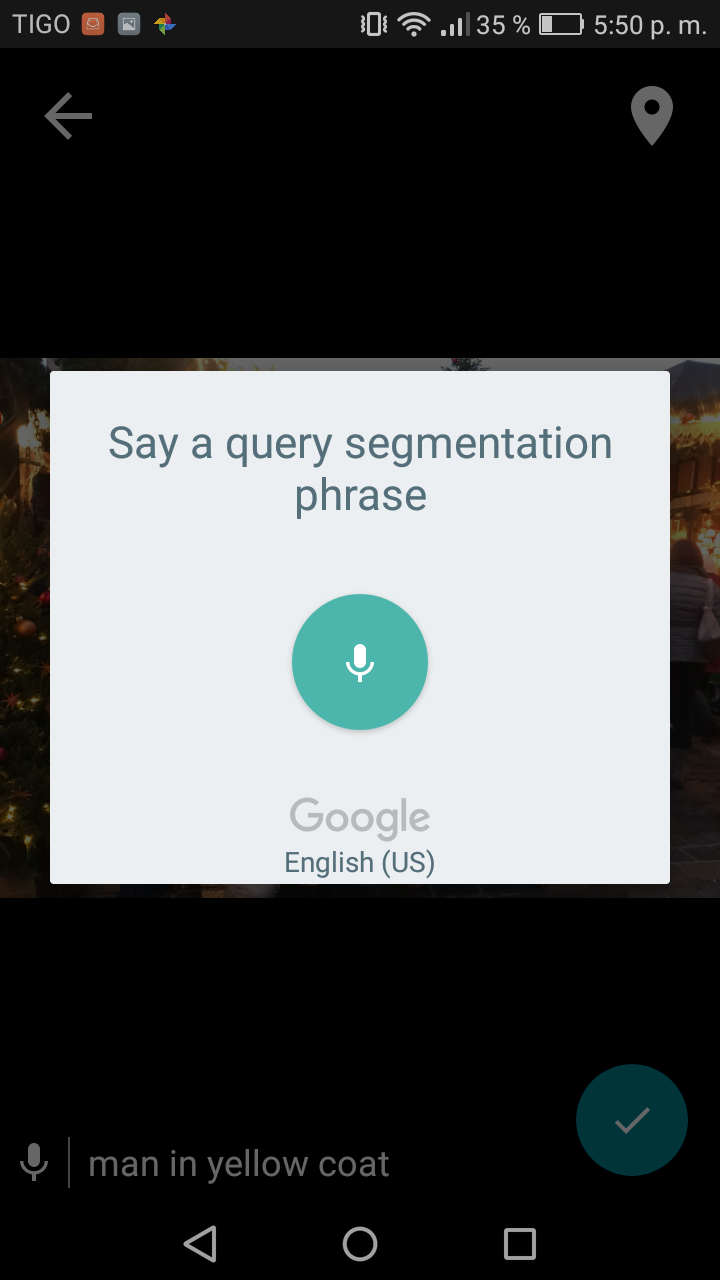
\includegraphics[width=\textwidth]{./figures/dmn_app/views/4.png}
    \subcaption{Use case \ref{subcase:query_input}: Query input via speech recognition using the microphone}
    \label{subfig:mic_input}
    \end{subfigure}
    
    \begin{subfigure}[b]{\columnwidth}
            \centering
            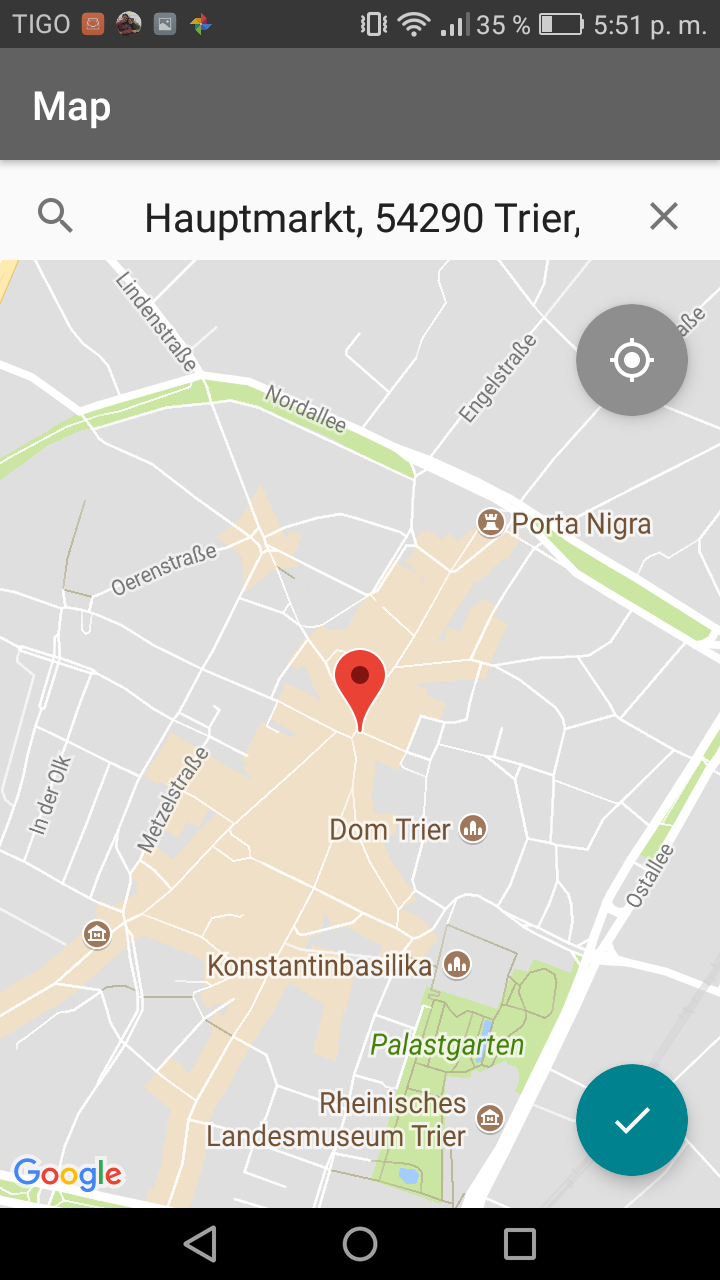
\includegraphics[width=\textwidth]{./figures/dmn_app/views/5.png}
    \subcaption{Use case \ref{subcase:gps}: Get user localization based on current position/custom place name}
    \label{subfig:loc}
    \end{subfigure}
    \end{multicols}
    
    \caption{\ref{subfig:image_pre}: DMN image preview activity, \ref{subfig:mic_input}: Speech-to-text recognition services, \ref{subfig:loc}: Localization Activity}
    \label{Fig:Img_Pre}
\end{figure}

If the user decides to submit the request to the server, the application takes the selected image, compress it and encodes it as a binary Base64 string, which is then sent to the frontend server alongside the device UUID in the application and the query phrase via asynchronous HTTP using Volley\footnote{Android's native HTTP client implementation}.

After the image is processed by the backend server and the FCM notification arrives back to the device, the application proceeds to checkout the latest change on the Firebase store, as it should contain a new entry depicting the request sent, adds it to the local database to prevent downloading its results on the application next start. Then the application connects to S3 and retrieves the request input image and its results, which consists of a heatmap preview image and the actual raw pixel-wise segmentation probability mask. After completing the downloads, the application displays a \texttt{CardView} depicting the input image (Figure~\ref{subfig:entry_view}), alongside its query, timestamp and localization (if exists). Additionally, the preview card allows to show the mask heatmap thumbnail image, as depicted on Figure~\ref{subfig:mask_preview}.

\begin{figure}[!htbp]
    \centering
    \begin{multicols}{2}
    \begin{subfigure}[b]{\columnwidth}
            \centering
            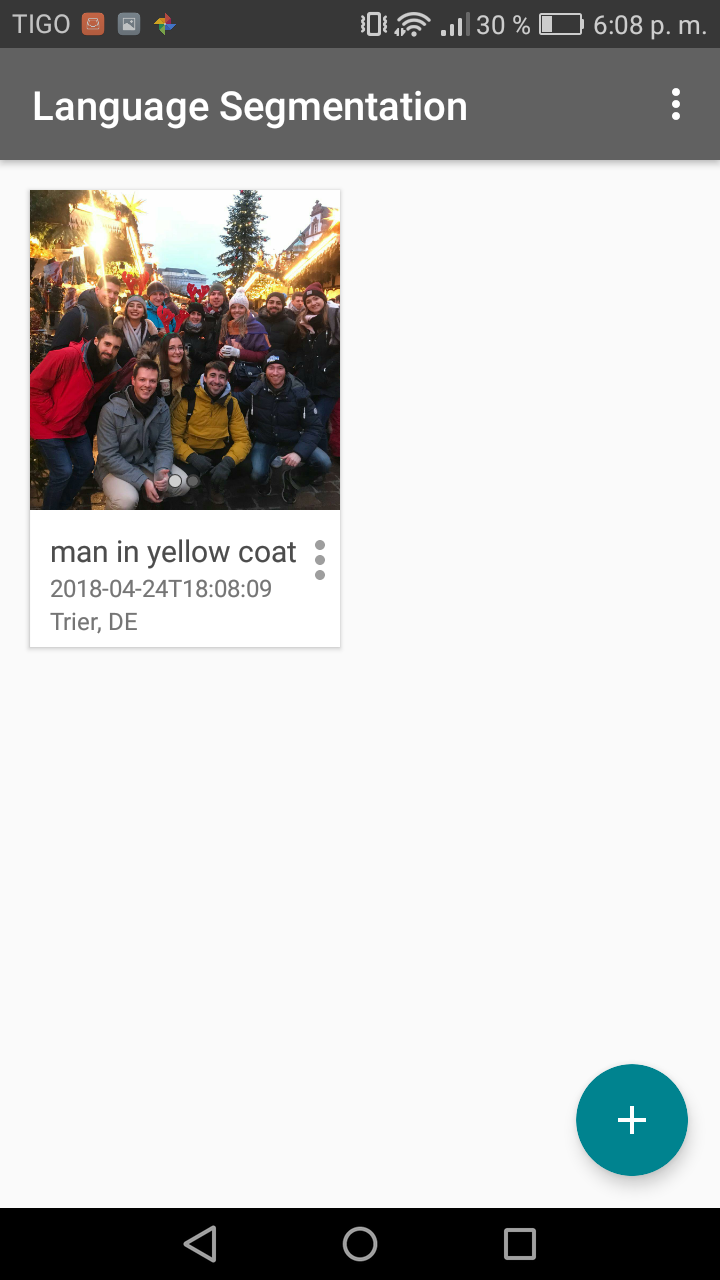
\includegraphics[width=\textwidth]{./figures/dmn_app/views/6.png}
    \subcaption{DMNApp main activity displaying a request response}
    \label{subfig:entry_view}
    \end{subfigure}
    
    \begin{subfigure}[b]{\columnwidth}
            \centering
            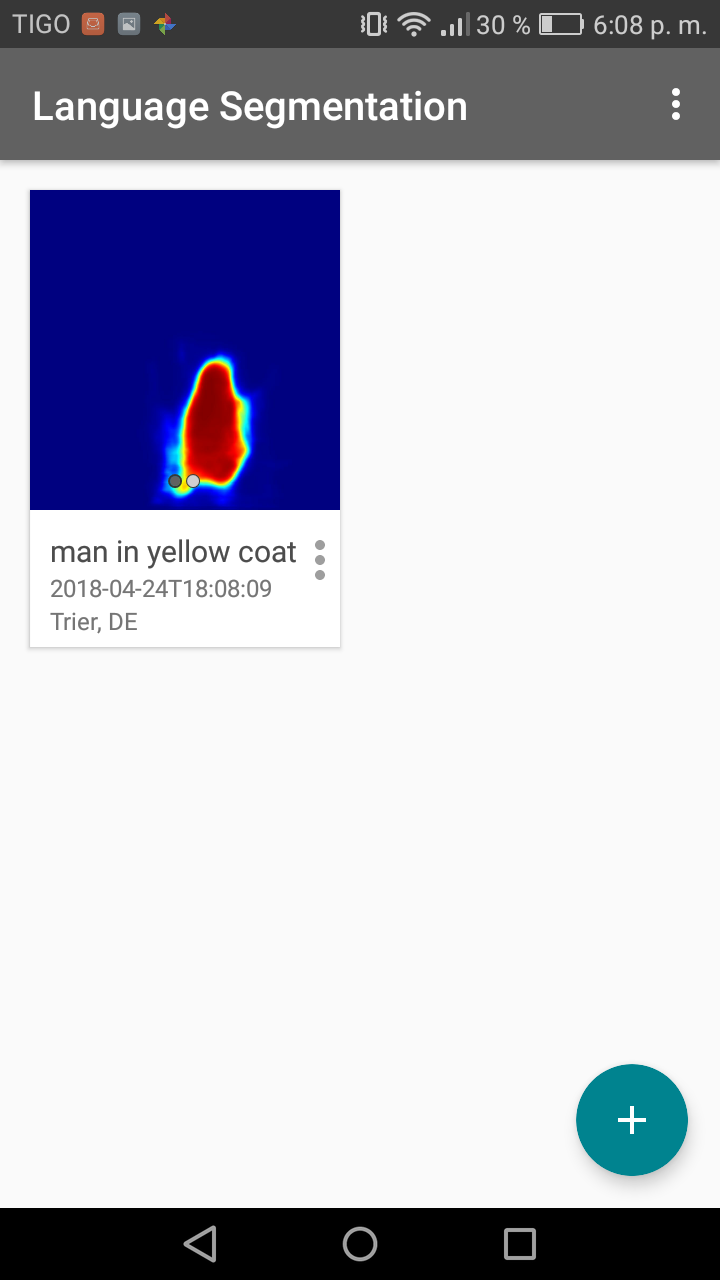
\includegraphics[width=\textwidth]{./figures/dmn_app/views/7.png}
    \subcaption{Request result mask heatmap preview on main activity}
    \label{subfig:mask_preview}
    \end{subfigure}
    \end{multicols}
    
    \caption{DMNApp main activity refresh after receiving a successful response for a request}
    \label{Fig:Main_Elem}
\end{figure}

If the user performs a click over a request response card, it will take her/him to the visualization activity (Figure~\ref{subfig:vis_mode}), where it is possible to observe a heatmap of the segmentation probability mask. To generate this view, the application must load the raw segmentation mask retrieved from S3 and interpret it byte-by-byte to load each pixel value\footnote{represented as float values of 64-bits} and transform it into an OpenCV \texttt{Mat} object, this object is cached for further processing. 

As OpenCV provides functions to map raw probabilities to colormap palettes, the application uses them to produce the images displayed on the heatmap visualization mode (Use case \ref{subcase:vis_heatmap}). Also, it is possible to display the mask using different colormaps (Use case \ref{subsubcase:colormap}), which can be changed by swiping left/right on the image, as it can be observed on Figure~\ref{subfig:colormap}.

\begin{figure}[!htbp]
    \centering
    \begin{multicols}{2}
    \begin{subfigure}[b]{\columnwidth}
            \centering
            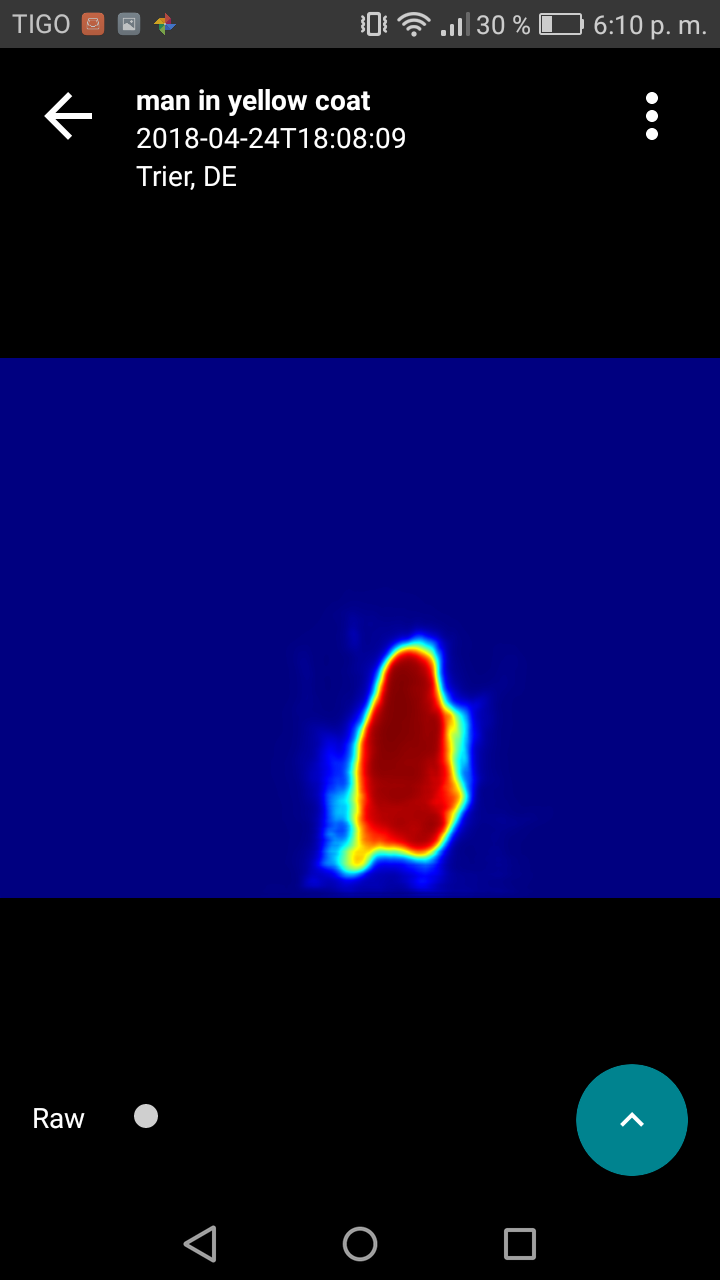
\includegraphics[width=\textwidth]{./figures/dmn_app/views/8.png}
    \subcaption{DMNApp mask visualization: Heatmap mode}
    \label{subfig:vis_mode}
    \end{subfigure}
    
    \begin{subfigure}[b]{\columnwidth}
            \centering
            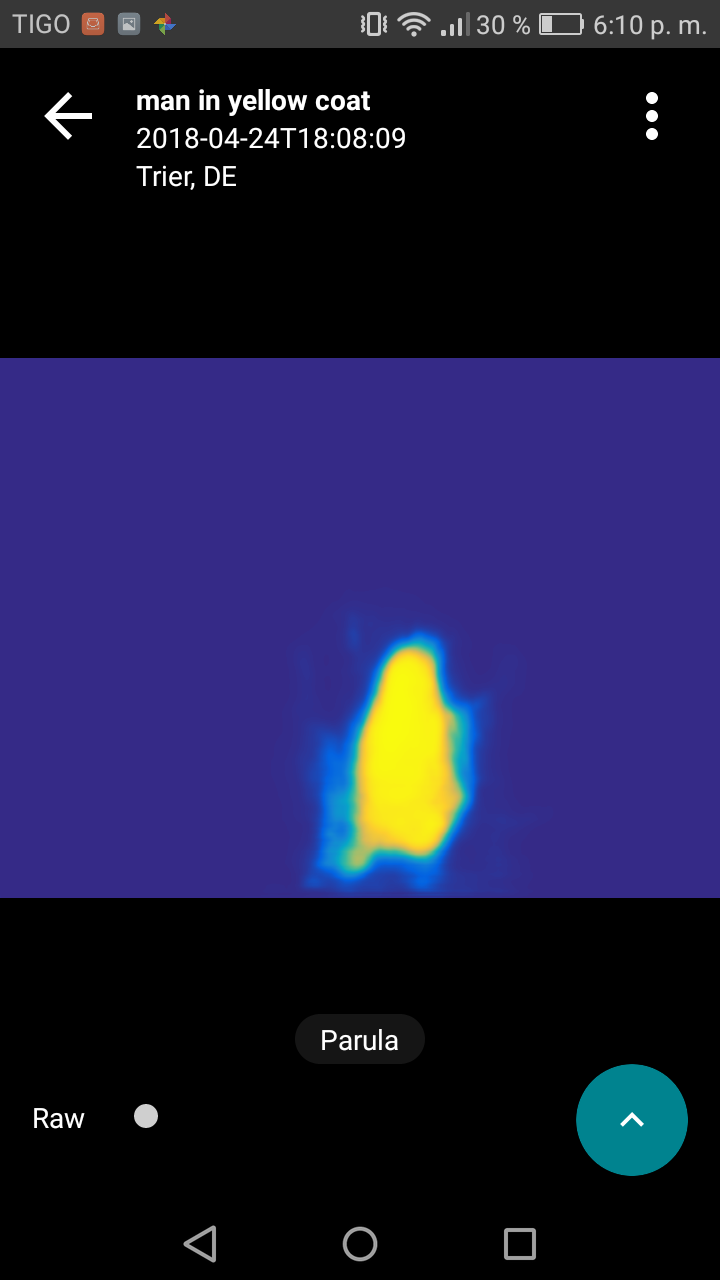
\includegraphics[width=\textwidth]{./figures/dmn_app/views/9.png}
    \subcaption{Display segmentation mask using different colormaps under heatmap mode}
    \label{subfig:colormap}
    \end{subfigure}
    \end{multicols}
    
    \caption{DMNApp heatmap mode visualization}
    \label{Fig:Vis_Heat}
\end{figure}